\subsubsection{ZDC Veto}\label{section:star_zdc_selection}
The~SDT trigger conditions imposed a veto on any signal in the~same-side ZDC. However, all MC samples do not contain ZDC simulation. To check the impact of this veto on the measurement, the total energy of neutral particles, such as $n$, $\gamma$, $\pi^{0}$, produced within ZDC acceptance ($|\eta|>6$) was measured using true-level PYTHIA~8~(SaS). In most of the events, the~energy measured on the proton side of the~IP is smaller than trigger thresholds (as shown in Fig.~\ref{fig:zdcSTAR}). Therefore, the~ZDC veto has a~negligible effect on the~analysis and ZDC simulation is not needed.


\begin{figure}[t!]
	%\vspace{-1cm}
	\centering
	\begin{subfigure}{.45\textwidth}
		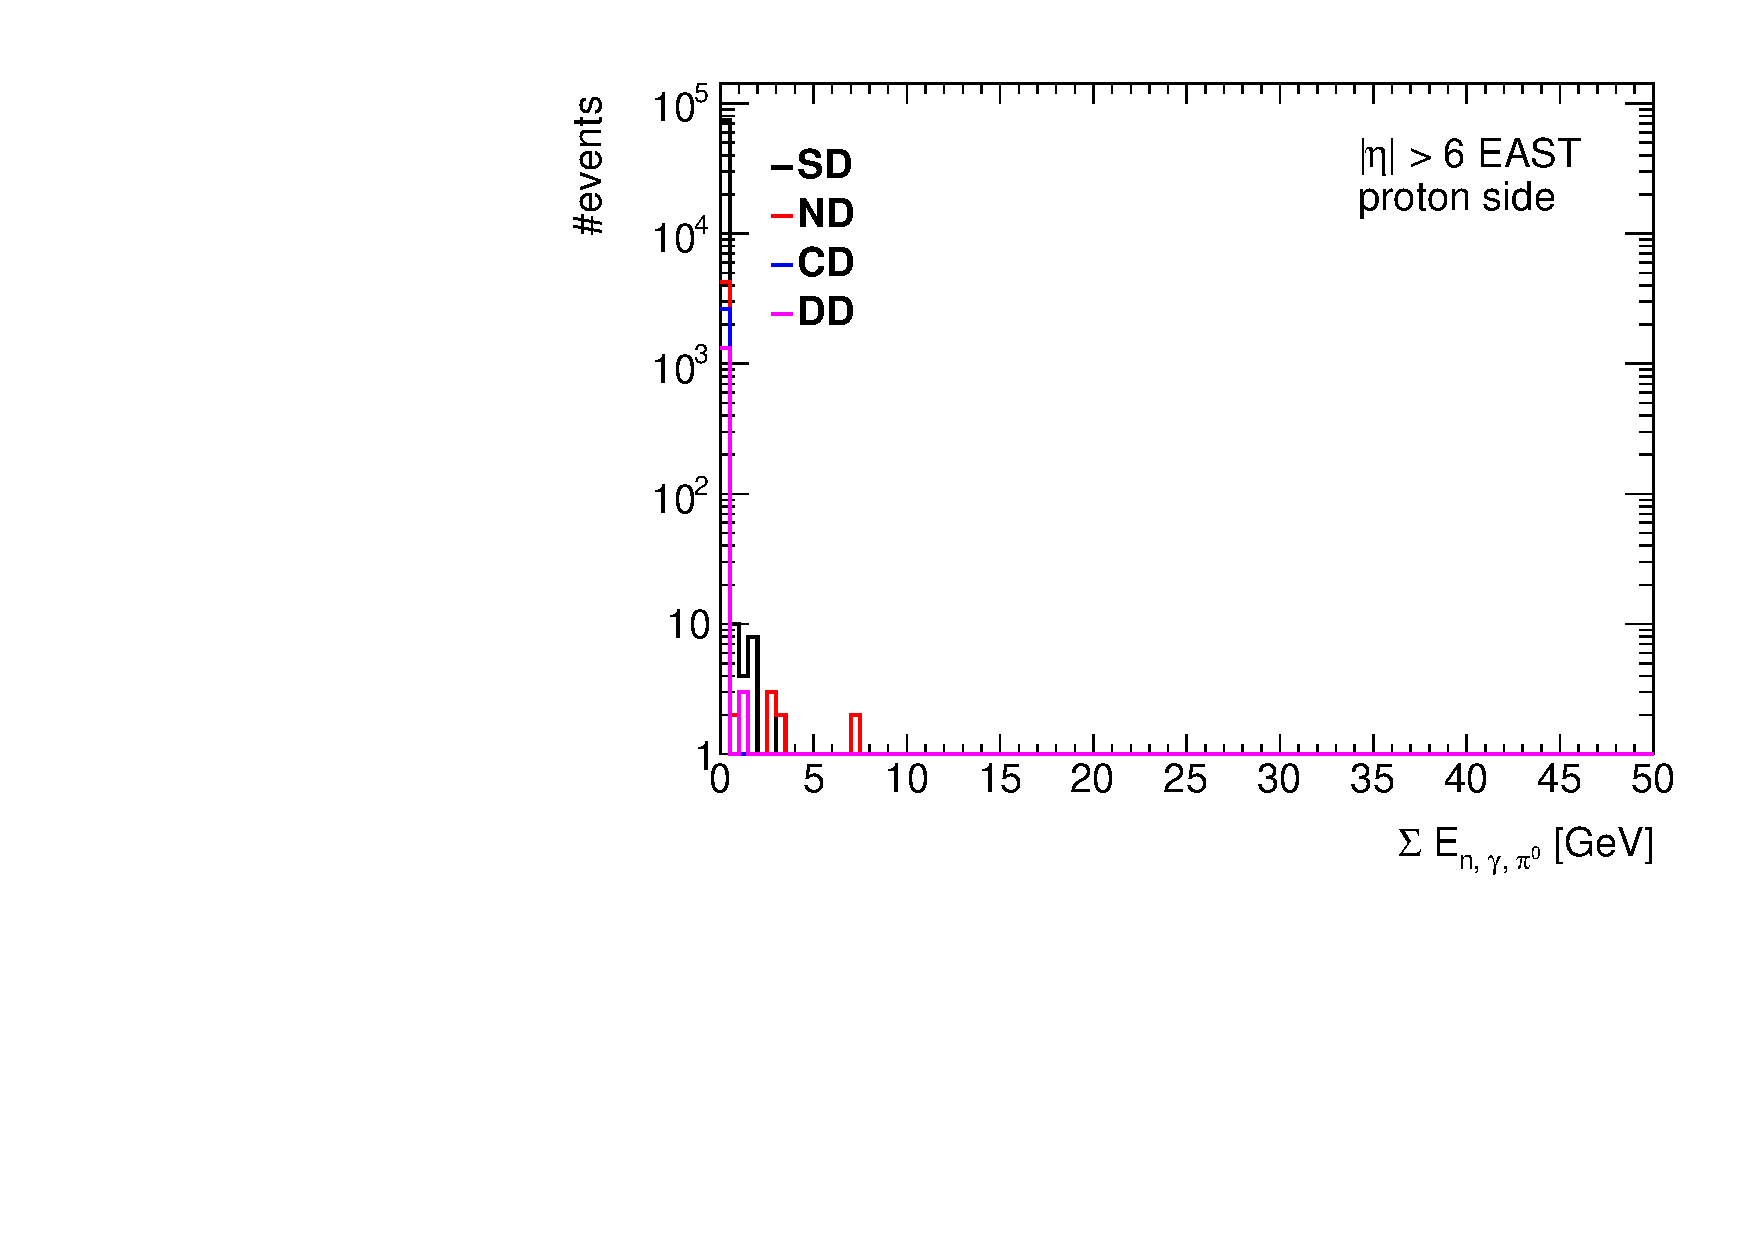
\includegraphics[width=\textwidth, page=1]{chapters/chrgSTAR/img/zdc/out.pdf}
		%\caption{}
	\end{subfigure}
	\begin{subfigure}{.45\textwidth}
		\includegraphics[width=\textwidth, page=2]{chapters/chrgSTAR/img/zdc/out.pdf}
		%\caption{}
	\end{subfigure}
	\begin{subfigure}{.45\textwidth}
		\includegraphics[width=\textwidth, page=3]{chapters/chrgSTAR/img/zdc/out.pdf}
		%\caption{}
	\end{subfigure}
	\begin{subfigure}{.45\textwidth}
		\includegraphics[width=\textwidth, page=4]{chapters/chrgSTAR/img/zdc/out.pdf}
		%\caption{}
	\end{subfigure}
	%\begin{minipage}{.45\textwidth}
		
		
		\caption{Total energy of neutral particles ($n$, $\gamma$, $\pi^{0}$) produced within ZDC acceptance ($|\eta|>6$) for events in which forward-scattered proton is on (top) west and (bottom) east side of the~IP. Distributions are presented separately for neutral particles produced on  (left) the proton and (right) opposite side of the IP. PYTHIA~8 predictions for different processes are shown as colour histograms. }
		\label{fig:zdcSTAR}
	%\end{minipage}
\end{figure}